
\section{Results}

\subsection{Filtering Process}

\begin{frame}
  \frametitle{Result - Scenario filtering}
  \center Video demo of the some filtered scenarios
\end{frame}


\subsection{Integration Method}

\begin{frame}
  \frametitle{Result - Discrete Integration Model}

  \begin{figure}

    \centering
    \begin{minipage}[b]{0.49\linewidth}

  \onslide<1, 2>{
        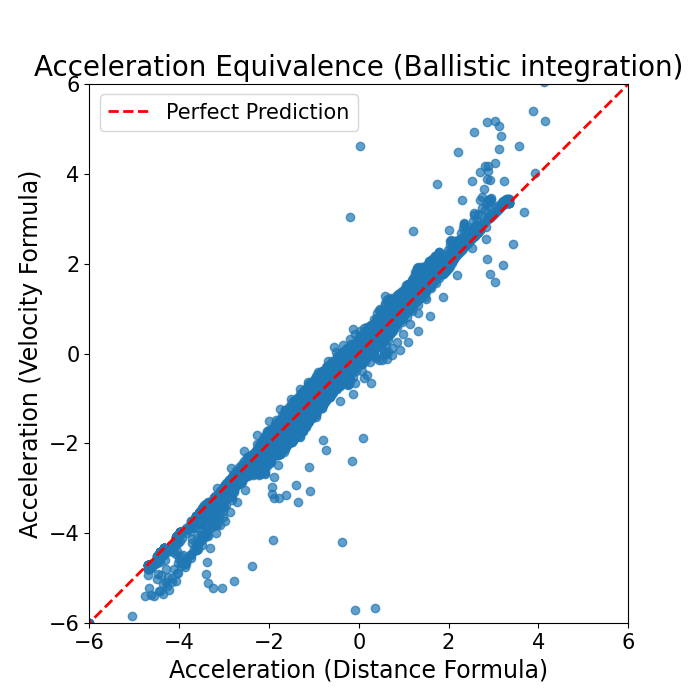
\includegraphics[width=\textwidth]{figures/graphs/Acceleration Equivalence (Ballistic integration).png}

        \centering \footnotesize MSE: 3.0786e+02
  }
    \end{minipage}
    \begin{minipage}[b]{0.49\linewidth}

  \onslide<2>{
        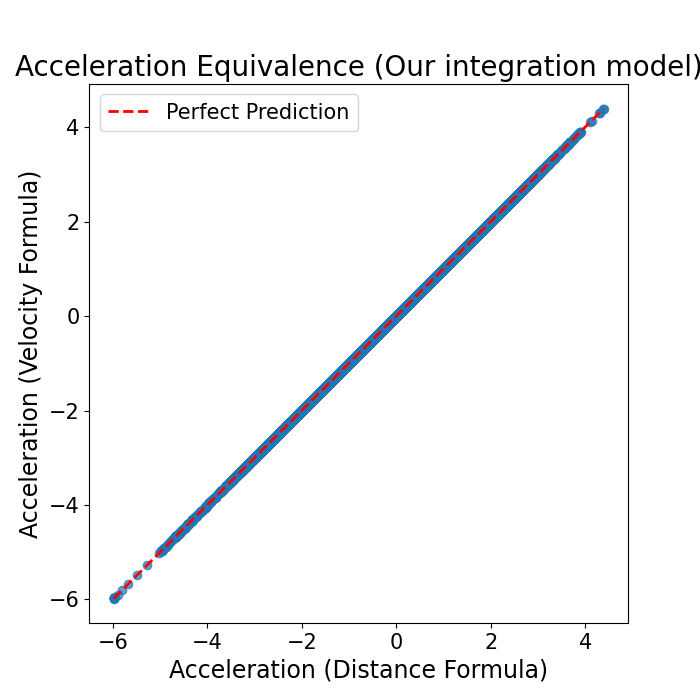
\includegraphics[width=\textwidth]{figures/graphs/Acceleration Equivalence (Our integration model).png}
        \centering \footnotesize MSE: 1.9220e-09
  }
    \end{minipage}
  \end{figure}
\end{frame}

\begin{frame}
  \frametitle{Result - Discrete Integration Model}
    Rearranging the formula to the distance and velocity gives us these results:
    \center \textit{Video demo of predicted car}
\end{frame}

